\documentclass[11pt, oneside]{article}
\usepackage{amssymb, url, natbib,enumerate}
\usepackage{graphicx,amssymb,amsfonts,amsmath,hyperref,cleveref,appendix}
\usepackage[top=1in,left=1in,right=1in,bottom=1in]{geometry}
\crefformat{footnote}{#2\footnotemark[#1]#3}
\bibliographystyle{aasjournal}
\newcommand\aap{A\&A}                % Astronomy and Astrophysics
\let\astap=\aap                          % alternative shortcut
\newcommand\aj{AJ}                   % Astronomical Journal (the)
\newcommand\aplett{Astrophys.~Lett.} % Astrophysics Letters
\newcommand\apj{ApJ}                 % Astrophysical Journal
\newcommand\apjl{ApJ}                % Astrophysical Journal, Letters
\let\apjlett=\apjl                       % alternative shortcut
\newcommand\apjs{ApJS}               % Astrophysical Journal, Supplement
\let\apjsupp=\apjs                       % alternative shortcut
\newcommand\apss{Ap\&SS}             % Astrophysics and Space Science
\newcommand\araa{ARA\&A}             % Annual Review of Astronomy and Astrophysics
\newcommand\jcap{J.~Cosmology Astropart. Phys.} % Journal of Cosmology and 
\newcommand\mnras{MNRAS}             % Monthly Notices of the Royal Astronomical 


\title{Memo: Phasing in \texttt{pyuvdata}}
\author{Garrett K. Keating, Bryna Hazelton, Matthew Kolopanis, Jonathan Pober, \\ on behalf of the \texttt{pyuvdata} team}
\date{\today}

\begin{document}
\maketitle

\section{Introduction}\label{sec:intro}
This memo contains an overview of how \texttt{pyuvdata} implements ``phasing'' -- the adjusting the phase of interferometric visibilities in order to synthesize an array that is coplanar to some position in the sky, for the purposes of imaging and other forms of analysis (e.g., power spectrum analysis). We include here an overview of the general process, as well as details on the specifics of how phasing is implemented within the \texttt{pyuvdata} software package, as well as the testing performed to verify the accuracy of these methods.


\subsection{A quick primer on celestial coordinates conventions}
A fundamental aspect of astronomy is being able to describe \emph{where} something is in the sky using a set of coordinates that can be readily translated into a position that an observer at any location on the Earth (or beyond!) can easily point their telescope to. Ground-based telescopes typically operate in ``horizontal'' coordinates, defined by a local horizon and where ``up'' is the direction of zenith. But because this horizon changes from location to location, it's more helpful to write coordinates in a frame that is \emph{not} location dependent, but instead is fixed by something in the sky, be it the position of stars, quasars, the Galaxy, etc. There are multiple coordinate systems that can be used, but the three generally most used in \texttt{pyuvdata} are FK5, ICRS, and ``apparent'' coordinates.

The ICRS\footnote{\url{https://en.wikipedia.org/wiki/International_Celestial_Reference_System_and_its_realizations}} frame is generally considered to be the current standard within astronomy, whose orientation is fixed by the positions of extragalactic radio sources. It replaced the previous standard -- the FK5\footnote{\url{https://en.wikipedia.org/wiki/Catalogues_of_Fundamental_Stars}} (also sometimes colloquially referred to as ``J2000'') frame, which was based on stellar positions -- though in most circumstances the coordinates between these two frames have only minor differences (typically of order 25 mas). The major exception to this arises from one of the fundamental differences between the FK5 and ICRS frames -- FK5 slowly rotates with time with respect to very distant (e.g., extragalactic) sources, whereas the ICRS frame is ``static''. The FK5 frame incorporates the precession of the Earth into the coordinate frame, which produces a shift of approximately an arcminute per year in the position of the celestial poles. As such, it is necessary to specify the epoch/time at which the FK5 coordinate system is being evaluated, the standard being the Julian year 2000.0 (``J2000'') epoch. Note that the FK5 frame is defined by the mean equinox at a given time -- where ``mean'' means that short-term variations such as nutation, polar motion, etc. are ``averaged over'' (i.e., the frame only accounts for changes due to precession, but not nutation or other terms).

In contrast, the apparent frame accounts for everything -- both long-term variations like precession, as well as shorter-term variations such as nutation, polar wobble, and stellar aberration. It is very similar to horizontal coordinates (differing only by two matrix rotations), with the primary difference being that the apparent coordinate frame is aligned to the rotation axis of the Earth  -- e.g., zenith for the observer can easily be defined in the apparent frame, with the right ascension equal to the local apparent sidereal time (LAST) and the declination equal to the latitude of the telescope site. Because it accounts for effects like the motion of the observer, it is both location and time dependent, making it less useful for things like publications, but it is very convenient frame for calculating the direction of a particular set of coordinates relative to an observer at some location and time. Given that interferometry relies on calculating the relative positions of different antennas as seen from the direction of the phase center, the apparent frame is quite convenient from a computational point of view, and is therefore the ``intermediate'' frame used within \texttt{pyuvdata} when defining the position of a phase center (which inside of a \emph{catalog} can be defined in any number of different frames, including FK5 and ICRS).

Like many other celestial frames, coordinates in the apparent frame are given as a right ascension and declination, with the relevant attributes stored as radians within \texttt{pyuvdata} objects. Apparent coordinates are sometimes colloquially referred to as ``topocentric coordinates'', though the latter more correctly refers to any coordinate system whose origin is a point on the surface of the Earth -- a description which would also include horizontal coordinates as well. 

\section{Conceptual description of phasing}\label{sec:concepts}
What is ``phasing''? Also sometimes referred to as ``fringe-tracking'' or ``fringe-stopping'', it is, in effect, the act of steering the center position of the interferometer, usually so that all Fourier modes measured by the interferometer are ``centered'' (i.e., at 0$^{\circ}$ position of the fringe) at some celestial position over the course of a track. There are a few benefits to this approach, not the least of which is that it makes Earth-rotation aperture synthesis possible, by way of enabling a sparse number of baselines can more completely fill in the synthesized aperture.

The way that phasing is achieved is to make the array ``co-planar'' with the plane tangent to the phase center, such that a planar wave traveling from some distant, celestial position arrives at all antennas at the same time. Of course in practice, the planar wave will end up \emph{physically} arriving at one telescope before another due to purely geometric effects -- e.g., light coming from a source that has just risen above the horizon will arrive at the eastern-most antennas within an array before it arrives at the western-most antennas. To compensate for this, one can introduce delays as part of the real-time correlation system (e.g., via FIFO buffers after digitization), or correct for the effect of the changing delays in post-processing -- the latter of which is done by \texttt{pyuvdata} (as well as other offline software processing packages).

Phasing consists of three critical steps:
\begin{enumerate}
    \item \textbf{Astrometry:} Calculate the position, from the observer's perspective, of the chosen phase center in the apparent coordinate frame. 
    \item \textbf{Rotation:} Calculate the distance between antennas, in the frame of reference where ``up'' (the $w$-direction) points toward the phase center, and the plane connecting ``up'' and ``north'' (the $w$ and $v$ directions, respectively) goes through the phase center position and the celestial poles. The projected distances in this frame are typically referred to as $uvw$-positions (or sometimes just $uvw$s).
    \item \textbf{Projection:} Correct for the differential delay in arrival of the light between the antennas of a given baseline (Figure~\ref{fig:simple_interferometer}), where that path difference is equal to the $w$-coordinate of the baseline. This is sometimes referred to as ``projecting'' the baseline or correcting for the geometric delay in time of arrival for different antennas of the light/planar wave originating at the phase center position.
\end{enumerate}

\begin{figure}[!t]
    \centering
    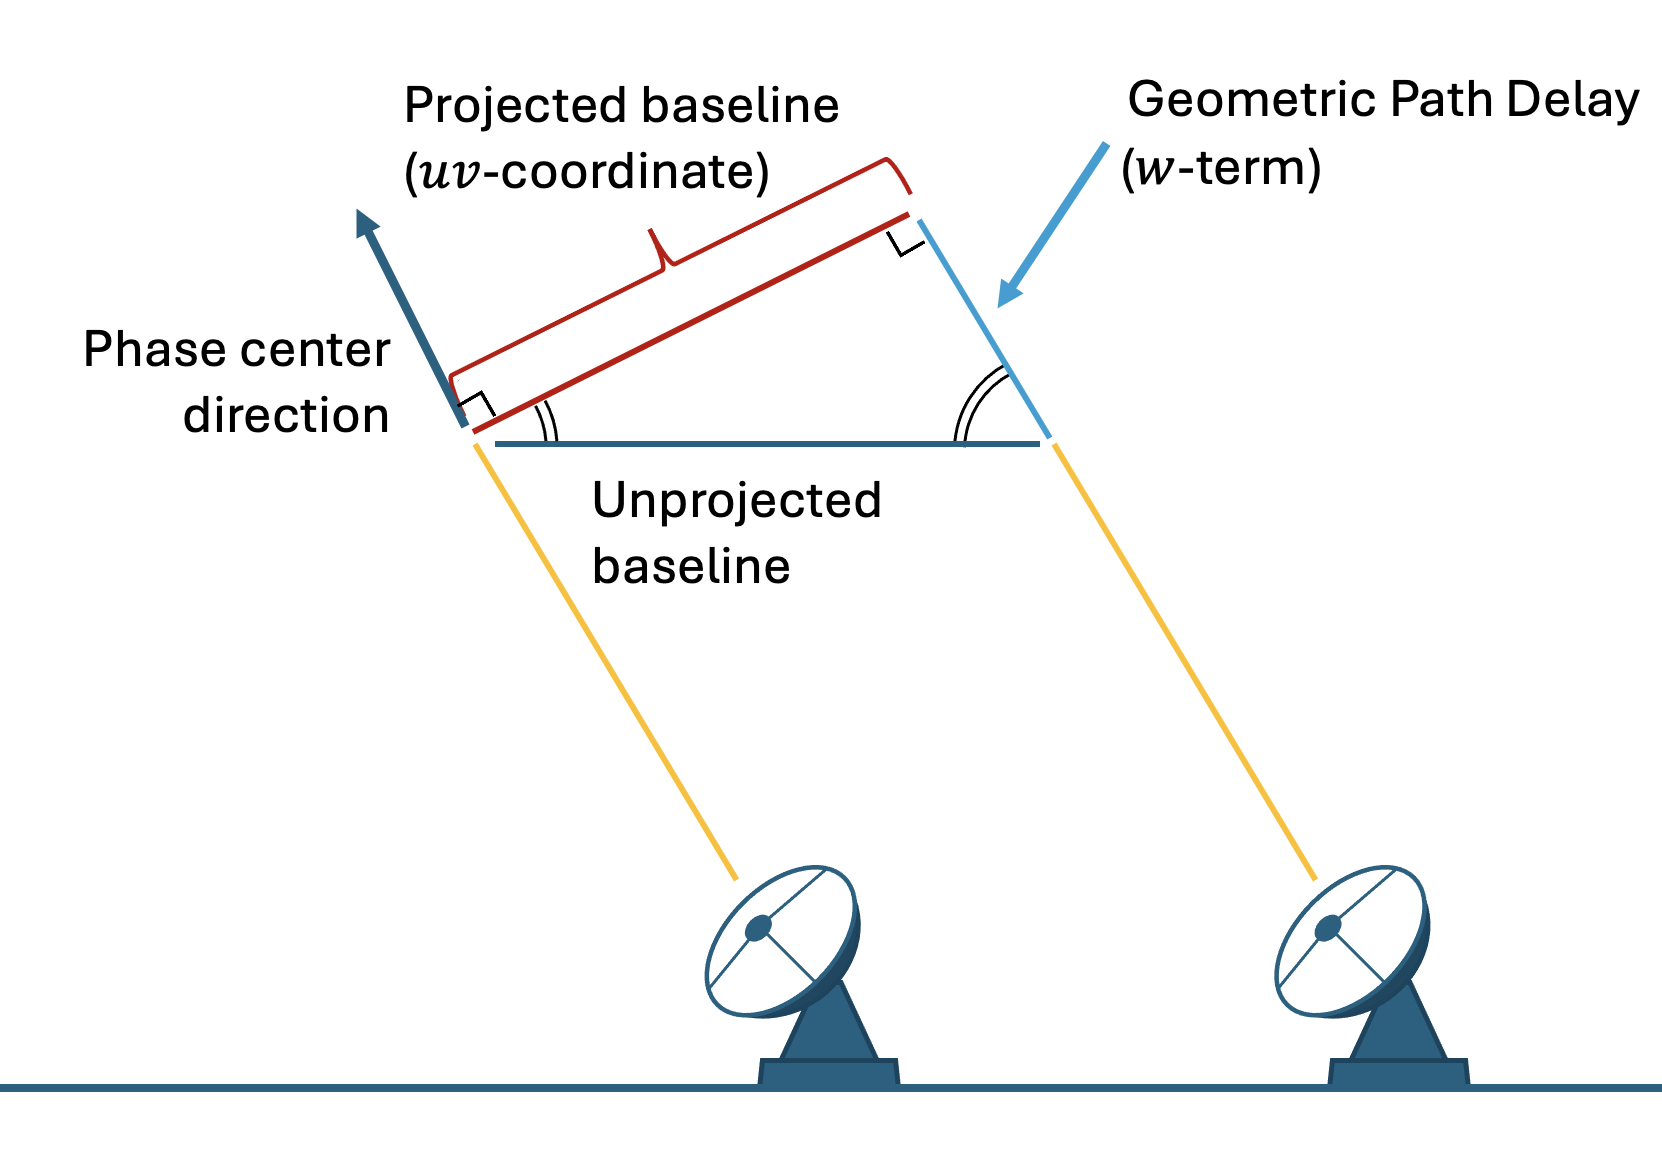
\includegraphics[width=0.75\textwidth]{simple_interferometer.png}
    \caption{Diagram of a simple, one-baseline interferometer. When performing imaging or other portions of analysis, one typically wants the array to be ``coplanar'' with the sky (i.e., on the plane perpendicular to the direction of the phase center), such that the light coming from some direction arrives at both antennas simultaneous. To synthesize this, one needs to compensate for the geometric path delay -- the extra light travel time due to the geometric configuration of the antennas relative to the array center. In \texttt{pyuvdata}, this correction is applied by applying a phase offset as a function of frequency for each baseline, which is proportional to the $w$-component of the $uvw$-coordinate of the baseline and the observing frequency. The remaining $uv$-component of the projected baseline vector is then generally used for imaging or other forms of analysis.}
    \label{fig:simple_interferometer}
\end{figure}

\begin{figure}[!t]
    \centering
    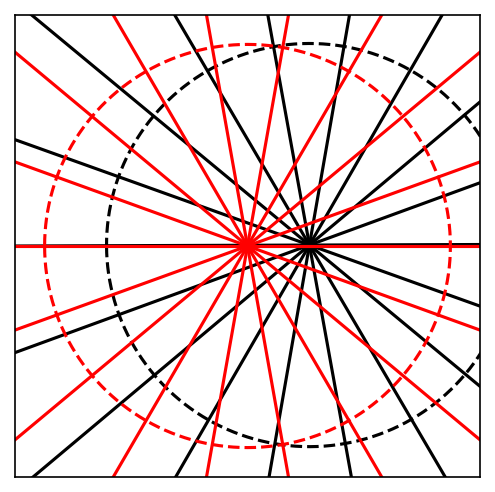
\includegraphics[width=0.45\textwidth]{ncp_icrs_app.png}
    \ 
    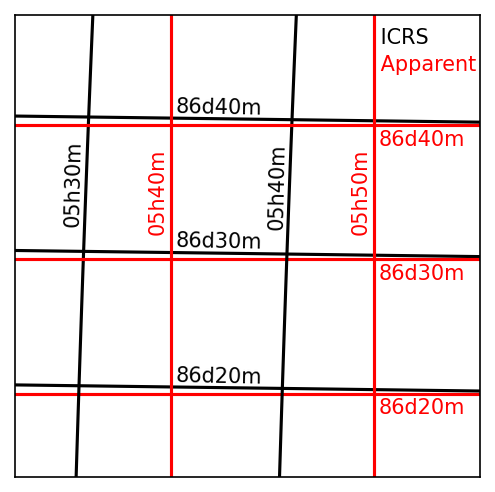
\includegraphics[width=0.45\textwidth]{app_icrs_frame_comp.png}
    \caption{\emph{Left}: Figure showing the region around the North Celestial Pole (NCP; $\delta=90^{\circ}$) of both ICRS (red) and apparent (black) coordinates, approximately 0.5$^{\circ}$ across. Solid lines show lines of constant right ascension, and dashed lines show lines of constant declination. In this region, the direction of the NCP -- which determines the direction of North on the map -- can change dramatically when considering the ICRS versus apparent NCP. If comparing interferometric maps to results in an ICRS frame, then one needs to rotate the map (either in the image domain or in the $uv$-domain) so that the direction of North is consistent. \texttt{pyuvdata} takes the latter approach of rotating the $uv$-coordinates so that the resultant image is appropriately oriented with the coordinate frame of the source -- be it ICRS, FK5, or other supported frame. \emph{Right}: Further away from the NCP, lines of constant right ascension and declination are closer to parallel, with the typical angle between them being a few tenths of a square degree.}
    \label{fig:coord_figures}
\end{figure}

\section{How phasing works in \texttt{pyuvdata}}\label{sec:methods}

\subsection{Astrometry Calculations}\label{ssec:astrometry}
The primary output of the astrometry stage is to calculate three outputs: the apparent right ascension (\texttt{UVData.phase\_center\_app\_ra}), the apparent declination (\texttt{UVData.phase\_center\_app\_dec}), and the apparent frame position angle (\texttt{UVData.phase\_center\_frame\_pa}). As mentioned above, the apparent coordinates are calculated from the frame of an observer on the surface, with effects like nutation and aberration already accounted for, such that all that's needed to ``find'' the position in the sky is knowledge of the latitude of the telescope (as recorded in \texttt{UVData.telescope\_location}) and the local apparent sidereal time (as recorded in \texttt{UVData.lst\_array}). The apparent frame PA is slightly different -- it measures the angle difference between north in the apparent frame and north in the specified coordinate frame (\texttt{cat\_frame} and \texttt{cat\_epoch}) at the phase center. 

These values are not needed for knowing where the phase center is from the perspective of the observer, but rather is information needed for orienting the apparent frame with the original coordinate frame that was provided (e.g., FK5, ICRS),  for reasons discussed further in Section~\ref{ssec:rotation}. The difference in orientation can be seen in Figure~\ref{fig:coord_figures} -- in the left panel, the north celestial pole of the ICRS and apparent frames can be seen in the center, with lines of right ascension (solid) showing the direction of North in these two frames. As you approach the NCP, these differences can be substantial, although they can still be significant further away from the pole (Figure~\ref{fig:coord_figures}; \emph{right}). This rotational ``misalignment'' is dominated by precession of the Earth, therefore also grows at a rate of approximately 1 arcminute a year.

Within \texttt{pyuvdata}, there are four different ``phase center types'' which are supported, though only three of them are relevant for discussion here: ``sidereal'', ``ephem'', and ``driftscan''.  Sidereal phase centers are those which can be described as a single longitude and latitude coordinate pair (e.g., RA and Dec) within a given celestial frame (e.g., FK5/J2000, FK4, Galactic). Ephem phase centers are those with whose positions are allowed to vary with time within a given celestial frame -- one such example being solar system bodies (e.g., Jupiter, Mercury, Vesta), which change position in the ICRS coordinate frame over time. Finally, ``driftscan'' are phase centers which remain at a fixed azimuth and elevation from the perspective of \texttt{UVData.telescope\_location}. The fourth phase center type -- ``unprojected'' -- has coordinates recorded in east-north-up (ENU) orientation, hence why it does not require astrometry (discussed more below).

With the exception of driftscan phase centers (which are simply translated from azimuth and elevation to apparent coordinates via a simple matrix rotation, provided by \texttt{erfa.ae2hd}), coordinates are first translated from their base coordinate system to the International Celestial Reference System (ICRS) via \texttt{astropy}.  Multiple coordinate frames are supported in this conversion, including FK5 (J2000), FK4 (B1950), and Galactic.

The intermediate ICRS coordinates are then translated to apparent coordinates -- that is, coordinates as seen by an observer at the position of \texttt{UVData.telescope\_location} -- via the \texttt{utils.transform\_icrs\_to\_app} method. Coordinate translation accounts for effects like precession and nutation, which track the meandering of the rotation axis of the Earth (relative to a fixed celestial frame), as well as stellar aberration (both annual and diurnal terms), which arises from the relativistic shifting of the sky due to the motion of the observer. Additionally, the method accounts for polar motion -- the small drifting difference between the pole position as defined by the International Terrestrial Reference Frame (ITRF; which \texttt{UVData.telescope\_location} is listed in) and the rotational axis of the Earth.

There are three underlying astrometry packages that can be used for transforming ICRS to apparent coordinates: \texttt{astropy}, \texttt{pyerfa}, and \texttt{novas}.  There are subtle differences in implementation, that may be of interest to expert users:

\begin{itemize}
\item{\texttt{pyerfa}}: A Python-based implementation of the ERFA software package, which is the core library used by \texttt{astropy} in its coordinate transformations. Coordinate rotations are implemented through the method \texttt{erfa.atco13}, and LSTs through \texttt{erfa.gst06a} (the output of which is modified to account for secular polar drift and the observer meridian relative to Greenwich meridian). This implementation is the fastest, although some low-level astrometry effects do not appear to be accounted for, such as Free Core Nutation (FCN; the misalignment between the rotational axis of the Earth's core versus the mantle layer). This can produce errors of order 0.1 mas, which is well below the tolerance required.

\item{\texttt{astropy}}: The \texttt{astropy} software package is one of the core libraries for \texttt{pyuvdata}, which can be used for calculating apparent coordinate positions, and is the sole package used for conversion between different celestial coordinate frames. \texttt{astropy} does not have a frame that corresponds to the apparent frame per se, but does allow for the calculation of horizontal coordinates (azimuth and elevation), which are straightforward to translate to apparent coordinates via matrix rotation knowing the observe latitude and LAST. Like \texttt{pyerfa}, there is no apparent handling of FCN. This implementation is about 50\% slower than \texttt{pyerfa}, although is generally quite consistent with the results of that package.

\item{\texttt{novas}}: A Python-based implementation of the US Naval Observatory NOVAS software package. Although it is the slowest of the three packages (roughly 3x slower than \texttt{pyerfa}), it does include some higher precision astrometry handling (such as FCN) which \textit{hypothetically} would make it the most accurate package, though users should be aware that the typical errors from IERS parameters used for these corrections are of order 0.1 mas (i.e., similar to the magnitude of the correction).
\end{itemize}

It is important to note that there is a discrepancy between \texttt{novas}-generated coordinates and those generated by the other two packages, of order 100--200 {\textmu}as. This difference is generally small enough to be insignificant for most application, and when using LSTs calculated by \texttt{novas} the difference in calculated position (in terms of horizontal coordinates) reduces by an order of magnitude. To that end, it is often best practice to use the same package for both calculating the LSTs and for calculating astrometric positions.

\subsection{Rotation to $uvw$}\label{ssec:rotation}
Once the astrometry calculations are complete, there are two potential paths toward calculating the $uvw$-coordinates, though we'll focus on the more typical path, which uses the antenna positions, $\mathbf{r}_{\rm ant}$ (as recorded in \texttt{UVData.antenna\_positions})\footnote{The alternative path works with the previously calculated \texttt{UVData.uvw\_array}, with the previously applied rotations removed, such that the projected baseline positions are measured relative to the line connecting 0$^\circ$ latitude and longitude and the Earth center, after which the rotations mentioned below are applied. Thanks to the commutative properties of matrices, this is mathematically equivalent to rotating the antenna positions first before differencing them to get the relative baseline positions.}. In total, we have three rotations to perform. We will denote these as $\mathcal{R}_{a,b}$, which is the rotation matrix about axis $a$ by amount $b$. Inside of a \texttt{UVData} object, the antenna positions are recorded in ECEF coordinates (or the lunar equivalent) relative to the \texttt{UVData.telescope\_location}, such that the array is oriented along the line that connects the center of the Earth to the position at 0$^\circ$ latitude and longitude. We'll refer to the plane that spans this direction and the northern pole as the Greenwich meridian. Therefore, in order to calculate the projected baselines, one needs to know the Greenwich Hour Angle (GHA) -- the separation between the Greenwich meridian and the meridian that goes through the phase center position and the north pole. This is relatively easy to calculate as:

\begin{eqnarray}
{\rm GHA} &=& {\rm GAST} - \alpha_{\rm PC}, \\
          &=& ({\rm LAST} - \theta_{\rm tel}) - \alpha_{\rm PC},
\end{eqnarray}
where GAST is the Greenwich apparent sidereal time, LAST is the local apparent sidereal time, $\alpha_{\rm PC}$ is the apparent right ascension of the phase center, and $\theta_{\rm tel}$ is the telescope longitude (where negative values correspond to Western hemisphere position). The rotation applied to align the array to the phase center meridian can thus be written as $\mathcal{R}_{\textrm{GHA}, z}$. After this first rotation is applied, as second rotation is performed to align the source declination to the x-axis of the frame, which can simply be written as $\mathcal{R}_{\delta_{\rm PC}, y}$, where $\delta_{\rm PC}$ is the phase center declination.

There is a final rotation that is applied, the need for which arises from a fairly simple question: what direction do we call ``north'' in our images? When we calculated our $uvw$-coordinates, we did so with north aligned to the celestial intermediate pole, or rather aligned to the \emph{current} rotational axis of the Earth. But due to precession and nutation (and to a much smaller degree, stellar aberration effects), this wanders by about 50 arcseconds per year\footnote{\url{https://en.wikipedia.org/wiki/Axial_precession}}, which means there is a field rotation that is of order tens of arcminutes field rotation of a measurement taken as of the time of writing this memo (2024) versus that taken at the beginning of the millennium. While a fairly subtle effect, this field rotation can be significant (particular when combining widely separated epochs of data or when comparing with non-interferometric data which have had field rotation effects removed).  Therefore, to compensate for this, the calculated $uvw$-positions are rotated one more time around the $w$-axis, by an amount which is recorded in the attribute \texttt{UVData.phase\_center\_frame\_pa}. This rotation aligns the $v$-axis of the $uvw$ domain such that it points toward north in the catalog frame of the object -- typically ICRS or J2000, but this can be any of the supported frames. This rotation can be written as $\mathcal{R}_{\phi_{\rm FPA},x}$.

Taken all together, the projected baseline vectors, $\mathbf{r}^{\prime}$, can be represented as:
\begin{equation}
\mathbf{r}^{\prime} = \mathcal{R}_{\phi_{\rm FPA},x} \mathcal{R}_{\delta_{\rm PC}, y} \mathcal{R}_{\textrm{GHA}, z} \mathbf{r}_{\rm ant}
\end{equation}
\subsection{Projection}\label{ssec:projection}
Once the $uvw$-coordinates are calculated, delay compensation for the $w$-projected distance is relatively straightforward, where the following per-visibility phase correction, $\phi^{\prime}$ is applied:
\begin{equation}\label{eqn:projection}
\phi^{\prime} = e^{-2i\pi\Delta w / \lambda_{\rm obs}},
\end{equation}
where $\Delta$w is the difference in $w$-projected distance (between the new and old phase center) for a given visibility, and $\lambda_{\rm obs}$ is the wavelength of the frequency channel the visibility belongs to. Note that when starting with unprojected data, no phase term has been applied, so $\Delta w$ is the full distance from the baseline pair to the plane, while if the data has been previously projected $\Delta w$ is the distance from the previous phase plane to the new phase plane. Delay corrections are applied using the observed frequency, as stored in \texttt{UVData.freq\_array}, versus the rest-frame frequency of the object in question, which is not accounted for by pyuvdata.

One final note -- all of the above assumes ``far-field'' objects, where the incoming wavefront can safely be presumed to be planar. Phasing for near-field objects (where the wavefront needs to be treated as spherical) is not yet supported, though exploratory development work is presently underway to support such phase centers.

\section{Limitations}\label{sec:limits}
There are a few limitations to the accuracy of the phasing methods within \texttt{pyuvdata}. For most users, these limitations are well below the threshold of significance for the data under analysis, but those doing very high resolution or astrometry measurements following the use of these methods should take heed of the information below.

\subsection{Precision Limits}
Accuracy of the astrometry is only guaranteed to $\sim1$ mas, tested at the highest precision level against data sets collected by the Submillimeter Array (SMA), which is generally sensitive to errors down to $\sim100$ mas. The level of precision in the results is guaranteed to be $\leq1$ mas, and in practice is generally closer to $\lesssim100$ {\textmu}as. This level of accuracy and precision is generally sufficient for all but the highest resolution interferometers, although users should be aware that these methods are not sufficiently accurate for VLBI-type phasing calculations (both for accuracy issues as well as some other effects discussed below). 

\subsection{Compensation for Decoherence}
Phasing in \texttt{pyuvdata} works by applying a frequency-dependent phase correction to the data to compensate for the differential delay between antennas. The phase correction is calculated at the center of the channel, but when phasing well away from the correlator phase center, decoherence is introduced due to the change in phase from one edge to another of a single frequency channel (sometimes called ``correlator squint'' or ``bandwidth smearing'') that \texttt{pyuvdata} does not compensate for. The exact impact depends on the details of the instrument, but the magnitude can be estimated as $\sim\Delta w \cdot \delta\nu / c$, where $\Delta w$ is the change in $w$-position of a given baseline, $\delta\nu$ is the channel width, and $c$ is the speed of light.

Similarly, corrections are also applied at the mid-point of an integration, though the phase of a given baseline may significantly evolve as the phase center changes position over time. This can give rise to a similar effect that described above (also referred to as ``time smearing''). The impact depends on a few parameters outside of the scope of this discussion, but a first order estimate of the impact can be calculated as $(\Delta w / \lambda_{\rm obs}) \cdot (\delta\tau / t_{\rm day})$, where $\lambda_{\rm obs}$ is the observed wavelength, $\delta\tau$ is the integration time, and $t_{\rm day})$ is the length of a day.

\subsection{Atmospheric effects}
When applying $w$-projection, \texttt{pyuvdata} methods calculate and apply corrections based on the difference in physical line-of-sight distance, with the light propagation speed effectively assumed to be that of free space. Of course, that approximation is not strictly true, since the index of refraction of air is slightly greater (by $\sim0.03\%$). As discussed in \cite{TMS}, this difference turns out to be negligible for antennas located at the same altitude and under conditions where plane-parallel approximations of the atmosphere hold (i.e., at elevations or array configurations where Earth-curvature effects are minimal relative to the wavelength of the observations), but outside of these circumstances, corrections must be made to compensate for the difference is the so-called ``excess path length''. Making such corrections requires knowledge of the ambient weather conditions and tools for calculating the index of refraction given those conditions -- neither of which \texttt{pyuvdata} has at the time of writing this memo. To first order, these effects are most likely to be significant when $\Delta h_{\rm max}\sim10^{3}\lambda_{\rm obs}$, where $\Delta h_{\rm max}$ is the maximum difference in altitude between antennas, and $\lambda_{\rm obs}$ is the observed wavelength. Note that many interferometers which apply phasing in real-time already compensate for these effects, such the impact of this when re-phasing data will small \emph{relative} to the magnitude of the overall shift, with the maximum possible error being $\sim10^{-4}$ times the magnitude of the difference in $w$-position.

\subsection{Static antenna positions}
Within \texttt{pyuvdata}, antenna positions are treated as static, relative to some fixed point on the surface of the Earth/Moon rotating about some axis\footnote{This can drift with time due to ``polar wobble'', among other effects, which is accounted for in astrometric calculations.}. This is obviously unsuitable for antennas which are not affixed to the ground (looking at you, space VLBI aficionados), but this also turns out to be untrue even for ground base instruments due to tidal effects, which on Earth can cause displacements of up to 55 cm. For most arrays, these effects are ``common mode'' -- they affect all antennas in the same way -- but it can produce milliarcsecond-level effects which are not presently compensated for. As such, the \texttt{pyuvdata} phasing framework is likely not be suitable for VLBI applications.

\subsection{Relativistic $uv$-stretching}
To first order, stellar aberration is accounted for as part of basic astrometry calculations, wherein center phasing position is calculated to very high accuracy. But there is a second-order effect, where the image plane is relativistically ``stretched'' ever so slightly, which translate in the $u$ and $v$ coordinates being marginally misaligned to the reference coordinate system (typically ICRS). The impact of annual aberration generally does not exceed one part in $10^{4}$, with maximum impact seen for fields along the ecliptic. Diurnal aberration is generally limited to one part in $10^{6}$, with maximum impact seen for equatorial targets. In both cases, the impact is only significant when dealing with an interferometer with long baselines relative to its field of view, i.e. where $|\mathbf{B}_{\rm max}| \sim \xi D_{\rm ant}$, where $\mathbf{B}_{\rm max}$ is the maximum-length baseline vector, $D_{\rm ant}$ is the antenna diameter, and $\xi$ is the impact factor of the aberration (where $\xi=10^{4}$ for annual aberration, and $\xi=10^{6}$ for diurnal aberration).

\subsection{$w$-projection effects}
Finally, we note $uvw$-coordinates are only calculated for a central phase center position. Wide-field interferometers -- where the spherical curvature of the sky means that patches of sky \emph{away} from the phase center will be warped by non-coplanar effects -- require additional care in handling. While pyuvdata tools provide no explicit support for handling such effects, several analysis packages (e.g., FHD, \citealt{FHD}; WSClean, \citealt{WSClean}) that interface with \texttt{pyuvdata}-supported formats are capable of doing so. Additionally, the orientation of the $uvw$-coordinates are aligned to north only for the central phase center position, such that images subtending large angular distances (i.e., $>>1^{\circ}$) may require additional handling to align to any given coordinate frame.

\appendix
\section{Commonly Used Terms}\label{appx:glossary}
\begin{itemize}
    \item\textbf{Coordinate frame}: Frame of reference which describes and orients the celestial sphere, typically defined by an equinox (axis that goes through 0$^{\circ}$ and 180$^{\circ}$ longitude at $0^{\circ}$ latitude) and the celestial poles (axis which goes through $\pm90^{\circ}$). Frames can be either inertial (i.e., non-rotating) or non-inertial (i.g., rotating) -- the latter requires an epoch specifying \emph{when} the coordinate frame is being considered in order to map it to a given position on the sky.
    \item\textbf{Coordinate epoch}: Time describing when a given coordinate is being considered. This is typically used in two contexts. First, for non-inertial coordinate frames, such as FK5, it is used to calculate terms like the precession and nutation to orient the axes of the frame. Second, for sources with proper motion, it defines the ``starting point'' in time, in order to calculate the total angular offset (given by product of the time delta and the proper motion -- typically given in mas/yr) from the reference position.
    \item\textbf{Greenwich sidereal time (GST)}: Angle (typically described in units of hours, where 6 hours is 90$^{\circ}$) that describes the current rotational orientation of the Earth relative to a celestial frame. Greenwich lies on the ``prime meridian'' (i.e., at a longitude of $0^{\circ}$), hence the name. As an example, a source at a right ascension of 14h will appear overhead in Greenwich (at it's highest point in elevation; at either $0^{\circ}$ or $180^{\circ}$ azimuth) at 14h GST. GST has two variants: ``mean'', which where the celestial frame accounts of precession/long-term shifts but no other terms; and ``apparent'', where the smaller/faster terms are included such that the celestial frame is the ``apparent'' frame.
    \item\textbf{Local sidereal time}: The ``local'' version of the GST, which is simply the sum of the GST and the local longitude. 
    \item\textbf{Precession}: The slow, steady change of the axis of rotation of the Earth caused chiefly by the Sun and the Moon, whereby in the orbital plane, the rotation axis shifts azimuthally. This causes the axis of rotation (and coordinate frames that are aligned with this axis) to shift by approximately one degree per 72 years, with a cycle of approximately 26,000 years.
    \item\textbf{North Celestial Pole (NCP)}: The northernmost point on the sky, from the perspective of the reference frame (\emph{typically} aligned close to the axis of rotation for the Earth).
    \item\textbf{Nutation}: The ``fast'' change of the axis of rotation, dominated by the orbital plane of the moon changing over a period of approximately 19 years (leading to a shift of approximately 9 arcseconds). Multiple small terms ($\sim$ arcsecond magnitude) with short cycles (less than 100 years in length) are grouped into this, typically consisting of hundreds of terms.
    \item\textbf{Polar motion}: Change in position of the surface of the Earth relative to its rotational axis. This typically produces shifts of a few meters between coordinate frames where the surface of the Earth remains ``fixed'' (e.g., ITRS) and where its defined relative to the ever-changing rotational axis.
    \item\textbf{Stellar aberration}: Shift in apparent position of celestial sources due to the motion of the observer. This is typically broken into two components -- \emph{annual aberration}, which arises from the Earth's orbital motion and has a magnitude of $\sim20"$; and \emph{diurnal aberration}, which arises from the rotation of the Earth and has a magnitude of $\sim0.3"$. Note that while canonically referred to as ``stellar'' aberration, the effect applies to all celestial sources (including radio galaxies). 
\end{itemize}

\section{Verification of \texttt{pyuvdata} phasing methods}\label{appx:verify}
As part of standard unit testing, astrometry calculations are tested between the three primary software packages (NOVAS, ERFA, astropy), to check for consistency. Standard tests use a small range of dates starting with May 11, 2014 (JD 2456789.0), at ICRS coordinates $\alpha$=09h25m37.43612s $\delta$=+40d52m10.7709s. These values were chosen somewhat pseudo-randomly, although more detailed comparison with additional datasets (as discussed below) has verified that the astrometry is valid outside of just this particular position and time. ERFA and astropy are generally agree to within a few microarcseconds. NOVAS shows larger magnitudes of disagreement (of order 0.2 mas), although neglecting celestial pole offsets (which neither astropy or pyerfa currently account for) and accounting for differences in calculated LST, these differences shrink to of order 10s of microarcseconds. Unit testing for \texttt{pyuvdata} requires that these methods produce a consistent set of results to within 1 mas.

Astrometry calculations have also been compared against a select number of test data sets, including those from ATCA and CARMA (\verb!atca_miriad! and \verb!carma_miriad!), which contain apparent coordinates as part of their metadata. Astrometry appears to agree down to a level of approximately 200 mas, which is a larger than expected, though anecdotal reports indicate that these data sets may not have diurnal aberration accounted for, which is consistent with the discrepancy. Calculations have also been done against several SMA data sets, which uses the NOVAS library as part of real time calculations. Values from these data sets agree with \texttt{pyuvdata} calculated values to of order 1 mas.\footnote{An older test data set located in the repository shows discrepancies of order 200 mas, although was traced back to an incorrect application of polar wobble corrections.} Additional testing with SMA datasets show a similar level of agreement, with the primary limitation arising from minor errors in the recorded LST versus something intrinsic to the calculation itself.

$uvw$-coordinates have been similarly checked against an MWA data set\footnote{A detailed comparison can be found at \url{https://github.com/RadioAstronomySoftwareGroup/pyuvdata/files/6525743/new.phasing.pdf}}, where the calculated positions agree with the MWA Cotter\footnote{\url{https://github.com/MWATelescope/cotter}} derived positions to better than a part in $10^7$ (after accounting for the apparent lack of frame position angle rotation in the latter).

%\begin{thebibliography}{9}
%
%\bibitem{USNO}
%  George Kaplan,
%  \textit{USNO Circular 179},
%  \href{http://aa.usno.navy.mil/publications/docs/Circular\_179.php}{\url{http://aa.usno.navy.mil/publications/docs/Circular\_179.php}},
%  2005
% 
% \bibitem{kaplan1998}
%  George H. Kaplan, High-Precision Algorithms for Astrometry: A Comparison of Two Approaches,
%  \textsl{The Astronomical Journal}, 115, 1, 1998
%  url={http://stacks.iop.org/1538-3881/115/i=1/a=361},
%\end{thebibliography}

\bibliography{phasing}
 
\end{document}